%=============================================================================
% Thesis Template in LaTex
%
% File:  02-Grundlagen und Theorie -- Grundlagen
% Author(s): Cyrano Golliez <golliezc@student.ethz.ch>>
%            
%
% Creation:  27 Jan 2014
% Time-stamp: <Tue 2013-08-13 20:14 juergen>
%
% Copyright (c) 2014 Infrastructure Management Group (IMG)
%               http://ibi.ethz.ch
%
% More information on LaTeX: http://www.latex-project.org/
%=============================================================================

\chapter{Grundlagen und Theorie}
\label{chap:Grundlage}

Diese theoretischen Grundlagen sind anhand der Unterrichtsmaterialien des Kurs System Engineering HS 2019 von Prof. Dr. Brayn T. Adey, Dr. Craig Richmond und Dr. Clemens Kielhauser, erarbeitet worden. Der Grossteil der Inforamtionen beziehe ich aus dem Skript zum Kurs. Zur weiteren Vertiefung habe ich die von Dr. Claudio Martani zur Verfügung gestellten Materialien zur Anwendung der \textit{Real option methodology}, konsultiert.  

\section{Problemlösungsprozess}
\label{sec:Problemprozess}

Der Problemlösungsprozess ist eine universell einsetzbare Methodik, zur bestimmung der optimalen Lösung einers Problems. Anhand diesem systematischen Prozess kann gewährtleistet werden, dass bei der Optimierung eines Systems alle Aspekte zum richtigen Zeitpunkt berücksichtig werden. So wird sichergestellt, dass die Bedürfnisse der vom betrachteten System abhängigen Personen befriedigt werden und die Funktionalität der erarbeiteten Lösungsvarianten gewährleistet ist. (\cite{Adey2019}) 

\begin{figure}[h!]
	\centering
	\includegraphics[width=\textwidth]{figures/02-01-Problemlösungsprozess}
	\caption[Schritte des Problemklösungsprozess]{Schritte des Problemklösungsprozess aus (\cite{Adey2019})}
	\label{img:Problemlösung}
\end{figure}

Nachfolgend werden die in Abbildung \ref{img:Problemlösung} dargestellten Schritte des Problemlösungsprozess, anhand des Skript des Kurs System Engineering, kurz erläutert. 

\paragraph{Anstoss} In diesem Schritt des Problemlösungsprozess werden die Grenzen und wirkenden Mechanismen des Problemfelds identifiziert, ein allgemeines Verständnis für das Problem entwickelt und überprüft ob das richtige Problem angegangen wird. Dies erfolgt anhand der differenzierung zwischen Wunsch und Wirklichkeit und der bestimmung des Umfangs der Bedürfnisse nach einer geänderten Situation.

\paragraph{Situationsanalyse} Der Zweck einer Situationsanalyse ist einerseits die Basis für die konkretisierung der Ziele zu schaffen und andererseits das Problem und die Notwendigkeit einer Intervention zu identifizieren. Weiter sollen die Zusammenhänge zwischen den Ursachen und dem Problem untersucht werden. Dies erfolgt mit der strukturierten Abgrenzung des Problemfelds und einer detailierten Darstellung der Ausgangssituation sowie der Aufgabenstellung. Anhand der Begrenzung des Problemfelds, auf den Bereich des Systems der im Rahmen der Problemlösung optimiert werden soll und der geschaffenen Informationsbasis können die nachfolgenden Schritte durchgeführt werden. Wichtige in diesem Schritt, für die erfolgreiche Optimierung einer Problemstellung ist, die Bestimmung der Diskrepanz zwischen Wunsch und Wirklichkeit.

\paragraph{Formulierung der Ziele und Rahmenbedingungen} In diesem Schritt werden alle Ziele, Wünsche und Absichten der beteiligten Personen zusammengetragen und ausführlich beschrieben, was und in welchem Umfang erreicht werden soll. Diese Beschreibung soll möglichst vollständig, realistische und objektiv sowie präzise und verständlich fomuliert, sein. Ausserdem muss bei der Formulierung darauf geachtet werden, dass die Erfüllung der Ziele feststellbar und das setzen von Prioritäten möglich, ist. 
Die Ziele werden in die folgenden Kategorien unterteilt.

\paragraph{Generierung von möglichen Lösungen} Unter diesem Stichpunkt werden anhand der folgenden Schritte, mögliche Lösungen für die Erfüllung der Ziele generiert. In einem ersten Schritt wird das neu zugestaltende Objekt genauer untersucht und anschliessend erste Lösungsideen entworfen. In einem zweiten Schritt werden alle als untauglich erachteten Lösungsideen aussortiert und die verbleibenden zu möglichen Lösungsvarianten ausgearbeitet. 
Zum erstellen der möglichen Varianten gehört bereits eine erste systematische Analyse und eine darauf folgende Anpassung der Varianten.
Das konkretisierungsniveau der Varianten soll der Plannungsphase entsprechen, in der sich das Projekt befindet. Dieser Schritt erfordert viel Kreativität da mit einem vertretbaren Aufwand, eine Visualisierung und Beschreibung der Varianten erschaffen werden muss, die vom neutralen Betrachter verstanden werden kann. Dies bedeuted, dass er das angewandte Konzept, mit dem das Problem gelöst werden soll, erkennen kann.

\paragraph{Analyse von möglichen Lösungen} In dieser Phase des Problemlösungsprozess, werden die Lösungsvarianten auf allfällige Schwachstellen überprüft. Dieser Schritt ist insofern sehr wichtig, da er aufzeigt, ob ein Lösungskonzept den gestellten Anforderungen entspricht. Dies erfolgt durch die überprüfung der Varianten in Hinblick auf die Erfüllung aller Rahmenbedingungen und der Optimierung der Zielfunktion. 

\paragraph{Bewertung von möglichen Lösungen} Die Bewertung der Lösungen dient dazu, die am besten geeignete Variante zu ermitteln. Durch das systematische vergleichen der Lösungsvarianten, wird eine objektive Entscheidungsfindung ermöglicht. Eine solche Bewertung erfolgt zum Beispiel mit einer Optimierung oder mithilfe von Entscheidungsbäumen. 

\paragraph{Durchführung} Die Durchführung schliesst den Problemslösungsprozess ab und beinhaltet die Ausführung der Variante, die im Bewertungsprozess als die beste identifiziert wurde. Die Durchführung ist abhängig von der Phase in der sich das Projekt befindet, was bedeuted, dass die Durchführung z.B. der Start einer Detailstudie (nach der Vorstudie) oder der Bau der Lösungsvarianten(nach der Detailstudie), sein kann.

\section{Interessensgruppen}
\label{sec:Inter.gruppen}

Als Interessensgruppen werden die Einzelpersonen, Gruppen oder Organisationen definiert, die von einer Veränderung der öffentlichen Strassenbetroffen sind. Die Interessensgruppen können in zwei Stufen unterteilt werden. Die erste Stufe umfasst die Interessensgruppen, deren netto Nutzen maximiert werden soll.  Diese beinhaltet zum einen die Besitzer der Infrastruktur, sowie die Nutzer als auch die direkt und indirekt betroffenen Öffentlichkeit. Im Falle der zwei letztgenannten ist die Zuteilung von der Zeit abhängig. So kann eine Person beim befahren der Infrastruktur ein Nutzer und wenn er Zuhause, in seiner an die Infrastruktur angrenzenden Liegenschaft, ist, Teil der direkt betroffenen Öffentlichkeit sein. Die zweite Stufe beschreibt die Interessensgruppen, die von der maximierung des netto Nutzen der Interessensgruppen der ersten Stufe, beeinflusst werden. Diese werden, sofern sie nicht Teil einer Interessensgruppe der ersten Stufe sind, nicht weiter berücksichtig oder aber fals dies explizit gefordert wird.(\cite{Adeyetall2019})

\section{Zielfunktion}
\label{sec:Zielf}

Um die optimale Lösung zu bestimmen, können im Problemlösungsprozess mathematische Modelle verwendet werden. Viele der verwendeten Modelle, zur optimierung von Problemen, haben eine einheitliche Aufbau aus einer Zielfunktion, die es zu maximieren oder minimieren gilt, sowie aus Nebenbedingungen, die die Grenzen der Varianten definieren. Die Zielfunktion sowie die Nebenbedingungen können linear oder nichtlinear sein.
Bei der Analyse von Varianten ist ein sogenanntes Lineare Programm (LP) mit einer linearen Zielfunktion und lineare Nebenbedingungen, aufgrund dessen, dass es mit dem Computer einfach zu berechnen ist, äusserst hilfreich.
Die Maximierung oder Minimierung der Zielfunktion, bei welcher die Beziehung zwischen linker und rechter Seit der Nebenbedingung beliebige Formen annehmen kann, durch ein allgemeines LP-Problem ermöglicht. Bei der allgemeinen Formulierung eines LP werden alle linearen Ausdrücke auf die linke und alle konstanten Ausdrücke auf die rechte Seite des Vergleichszeichens geschrieben. \cite{Adey2019}

Nach \cite{Adey2019} erfolgt die Darstellung einer Zielfunktion gemäss Formel \ref{eg.02-01}.

\begin{equation}
Maximieren: Z = c_{1} \cdot x_{1} + c_{2} \cdot x_{2} + c_{3} \cdot x_{3} + \dots + c_{n} \cdot x_{n}
\label{eg.02-01}
\end{equation}

{\setstretch{0.6}
mit:
\begin{conditions}
 c_{j}	 		  &  Gewinn für jede Einheit der j-ten Aktivität \\
 x_{j} 		      &  Ausmass der j-ten Aktivität oder Entscheidung \\
 j \{1 \dots n \} &  Index der Aktivitäten oder Entscheidungen 
\end{conditions}
} 

\subsection*{Nebenbedingungen}

Gemäss (Adey et. all., 2019) sind die Nebenbedingungen der Versuch die Rahmenbedingungen mathematisch auszudrücken. Sie repräsentieren die Anzahl an Einheiten der Ressource i, die in allen Aktivitäten n konsumiert werden können. Die Nebenbedingungen werden wie folgt dargestellt:

\begin{equation}
\begin{aligned}
  a_{1,1} \cdot x_{1} +  a_{1,2} \cdot x_{2} +  a_{1,3} \cdot x_{3} + \dots +  a_{1,n} \cdot x_{n} &\leq b_{1} \\
  a_{2,1} \cdot x_{1} +  a_{2,2} \cdot x_{2} +  a_{2,3} \cdot x_{3} + \dots +  a_{2,n} \cdot x_{n} &\leq b_{2} \\
  																								   &\vdots     \\
  a_{m,1} \cdot x_{1} +  a_{m,2} \cdot x_{2} + a_{m,3} \cdot x_{3} + \dots + a_{m,n} \cdot x_{n} &\leq b_{m} 					
\end{aligned}
\end{equation}

{\setstretch{0.6}
mit:
\begin{conditions}
 a_{i,j}	 	   &  Koeffizient der j-ten Aktivität in der i-ten Nebenbedingung \\
 x_{j} 		       &  Ausmass der j-ten Aktivität oder Entscheidung \\
 b_{i} 			   &  Verfügbare Menge der Ressource i \\
 i\{1 \dots m\}    &  Index der Ressourcen \\
 j\{1 \dots n\}    &  Index der Aktivitäten oder Entscheidungen 
\end{conditions}
} 

\subsection*{Nichtnegativitätsbedingungen}

Gemäss (\cite{Adey2019}) verhindern Nichtnegativitätsbedingungen, dass negative Werte im Ergebnis vorkommen. Dies bedeutet, dass Aktivitäten nur zu einem positiven Mass oder gar nicht durchgeführt werden dürfen. Für jede Art von Ressource, die in einer Gruppe von Aktivitäten konsumiert wird, d.h. für $i=1,2,\dots m$ müssen diese Nebenbedingungen definiert werden. 

\begin{equation}
	x_{1} \geq 0, x_{2} \geq 0, x_{3} \geq 0, \dots, x_{n} \geq 0
\end{equation}

\newpage

\section{Entscheidungsbaum}
\label{sec:Decisiontree}

In einem Entscheidungsbaum werden alle Möglichkeiten, Entscheidungen und berücksichtigten Varianten des Entscheidungsprozess dargestellt. Dies soll dem Betrachter ermöglichen, nachzuvollziehen wieso eine Entscheidung getroffen wurde. Damit man die Ergebnisse des Entscheidungsbaums vergleichen kann, müssen einerseits die Unsicherheiten der betrachteten Szenarien bekannt sein und andererseits die Bewertung der Varianten anhand einer einheitlichen Skalierung erfolgen.

Ein Entscheidungsbaum besteht aus fünf Grundelementen, die nachfolgend anhand (\cite{Adey2019}) kurz erläutert werden.

\paragraph{Kosten bzw. Nutzen} stellen dar, was für die Entscheidung relevant ist. Um den Erwartungswert eines Szenario berechnen zu können, müssen alle die gleiche Masseinheit habe.

\paragraph{Wahrscheinlichkeiten} liegen immer zwischen 0 und 1, und stellen dar wie wahrscheinlich das Eintretten einer Möglichkeit ist. Der mit der Wahrscheinlichkeit gewichtete Wert, ist somit stets kleiner oder gleich dem ursprünglichen Wert. 

\paragraph{Entscheidungsknoten} sind durch quadratische Knoten gekennzeichnet, an welchen der Entscheidungsträger zwischen verschiedenen Varianten auswählen muss. An diesen Verzweigungen beeinflusst der Entscheidungsträger den Entscheidungsprozess mit der wahl einer Variante. Der Wert des Entscheidungsknoten wird auf der Summe aller eingehenden Zweige gebildet.

\paragraph{Möglichkeitsknoten} stellen Verzweigungen dar, bei denen unsicher ist, welche Szenario eintretten wird. Sie werden mit einem Kreis dargestellt, wobei die vom Kreis ausgehenden Linien die möglichen Entscheidungen darstellen. Diese Entscheidung kann der Entscheidungsträger nicht beeinflussen. 
Der Erwartungswert eines Möglichkeitsknoten ist die Summe der wahrscheinlichkeitsgewichteten Werte der verschiedenen Möglichkeiten eines Knoten. Folgen zwei Entscheidungsknoten aufeinander, ergibt sich am Ende des Pfades ein Kombination der Szenarien. Die Eintrittswahrscheinlichkeit eines kombinierten Szenarios berechnet sich aus der multiplikation der Wahrscheinlichkeiten entlang des Pfads. 

\paragraph{Blätter} symbolisieren durch ein gekipptes gleichseitiges Dreieck das Ende eines Pfades. An dieser Stelle werden die Gesamtkosten bzw. -nutzen eines möglichen Szenarios eingetragen.

\pagebreak

Die nachfolgenden Abbildung zeigt ein fiktives Beispiel eines Entscheidungsbaum im Rahmen einer Variantewahl.

\begin{figure}[h!]
	\centering
	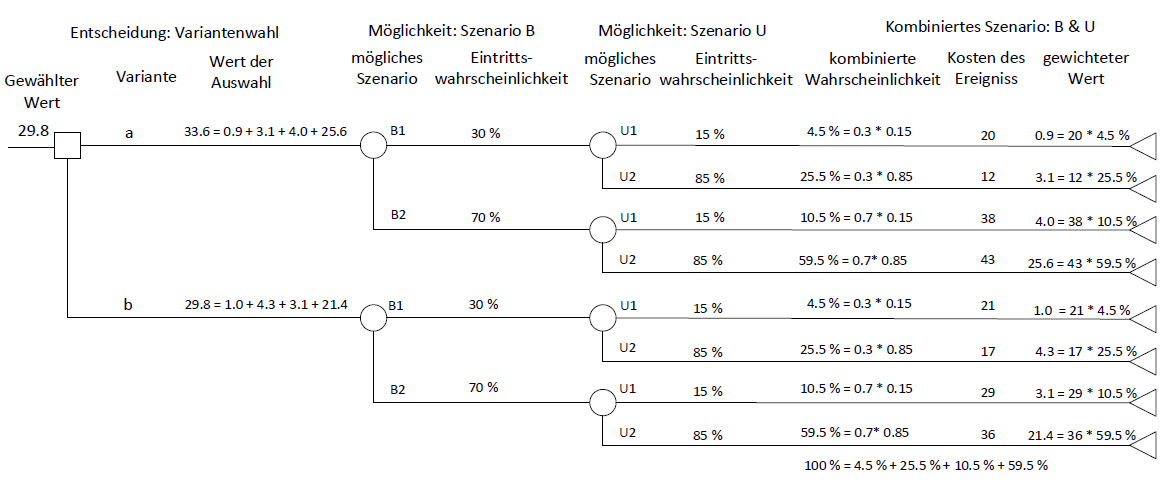
\includegraphics[width=\textwidth]{figures/02-02-EntscheidungsbaumBSP}
	\caption[Beispiel Entscheidungsbaum]{Beispiel eines Entscheidungsbaum}
	\label{img:Problemlösung}
\end{figure}

Gesucht wird die Variante, welche die geringsten zuerwartenden Kosten und somit das kleinste Risiko generiert. Die Berechnung der Kosten erfolgt in diesem Beispiel von rechts nach Links, wobei der zeitliche Verlauf der Entscheidungssituation von links nach rechts dargestellt wird. 

\section{Sensitivitätsanalyse}
\label{sec:Sensitivität}

Ein wichtiger Bestandteil der Kosten-Nutzen Analyse ist zu untersuchen, wie stark ein Ergebniss von den getroffenen Annahmen abhängt. Dies erfolgt anhand der sogenannten Sensitivitätsanalyse, die aufzeigt, ob das Ergebniss von den getroffenen Annahmen abhängt und wie robust das Ergebniss auf eine Variation der Parameter reagiert. \\
Die Sensitivitätsanalyse kann sowohl mit den Nebenbedingungen als auch mit der Zielfunktion durchgeführt werden. In beiden Fällen wird untersuche was passiert bei einer Veränderung der ursprünglichen Annahmen und in welchem Rahmen können die Parameter verändert werden, ohne das sich das ursprüngliche Ergebniss verändert. 
Diese Analyse ermöglicht es die Belastbarkeit der Ergebnisse, in einer allfälligen Diskussion der Variante, zu stärken. (\cite{Adey2019})

\pagebreak
 
\section{Real option methodology}
\label{sec:RealOption}

Die \textit{real option methodology} ist ein Vorgehen, um die optimale Variante einer Intervention, unter berücksichtigung von unsicheren zukünftigen Gegebenheiten, zu bestimmen. 
Die \textit{real option methodology} ermöglicht es, Varianten einer Infrastruktur Intervention zu erarbeiten, die auf zukünftige veränderliche Rahmenbedingungen vorbereitet sind. \\
So kann das einbeziehen von flexiblen Designs, im Prozess der Erschaffung einer Infrastrukturintervention, zusätzliche Vorteile generieren sowie zukünftige Risiken beseitigen.  \\
Weiter sollten Infrastrukturen über einen längeren Zeitraum hinweg, ihre Serviceleistung auf einem angemessenen Niveau erbringen könnne. Dies setzt vorraus, dass sich die Infrastruktur an veränderliche Bedingungen anpassen und die Bedürfnisse der Interessensgruppen über einen längeren Zeitraum erfüllen, kann. 
Mit dieser Methodik kann, unter Berücksichtigung von unsicheren Variablen wie zum Beispiel der Veränderung der Anzahl Nutzer oder der Baukosten, ermittelt werden, welches Design den netto Nutzen des Investors am meisten vergrössert. 
Das Design einer Infrastruktur anstatt star, flexible zu gestalten ist meistens sehr teuer. Diess lohnt sich nur dann, wenn die Anpassungskosten der Infrastruktur kleiner als die Mehrkosten des flexiblen Designs sind.
(\cite{Neufville2011}) (\cite{Esders2015}) \cite{Martani2018}




% ===========================================================================
% EOF
%

%%% Local Variables:
%%% mode: latex
%%% TeX-master: "../main"
%%% End:
